\section{Atividades}

Neste módulo, foram realizadas atividades práticas voltadas à proteção de
informações utilizando técnicas de segurança aplicadas no sistema operacional
Kali Linux. As tarefas envolveram o uso de esteganografia para ocultar
mensagens em imagens, além da aplicação de técnicas de ofuscação de código em
Python para dificultar a compreensão do código fonte original.

Também foram explorados mecanismos de criptografia simétrica utilizando
diferentes algoritmos disponíveis no OpenSSL, como AES-256, 3DES e Blowfish,
permitindo compreender na prática como arquivos podem ser cifrados e
posteriormente decifrados. O objetivo foi demonstrar métodos utilizados para
proteger dados e dificultar o acesso não autorizado às informações.

\newpage

\question[Atividade 8.1]{Esteganografia no Kali Linux}

\begin{figure}[H]
\centering
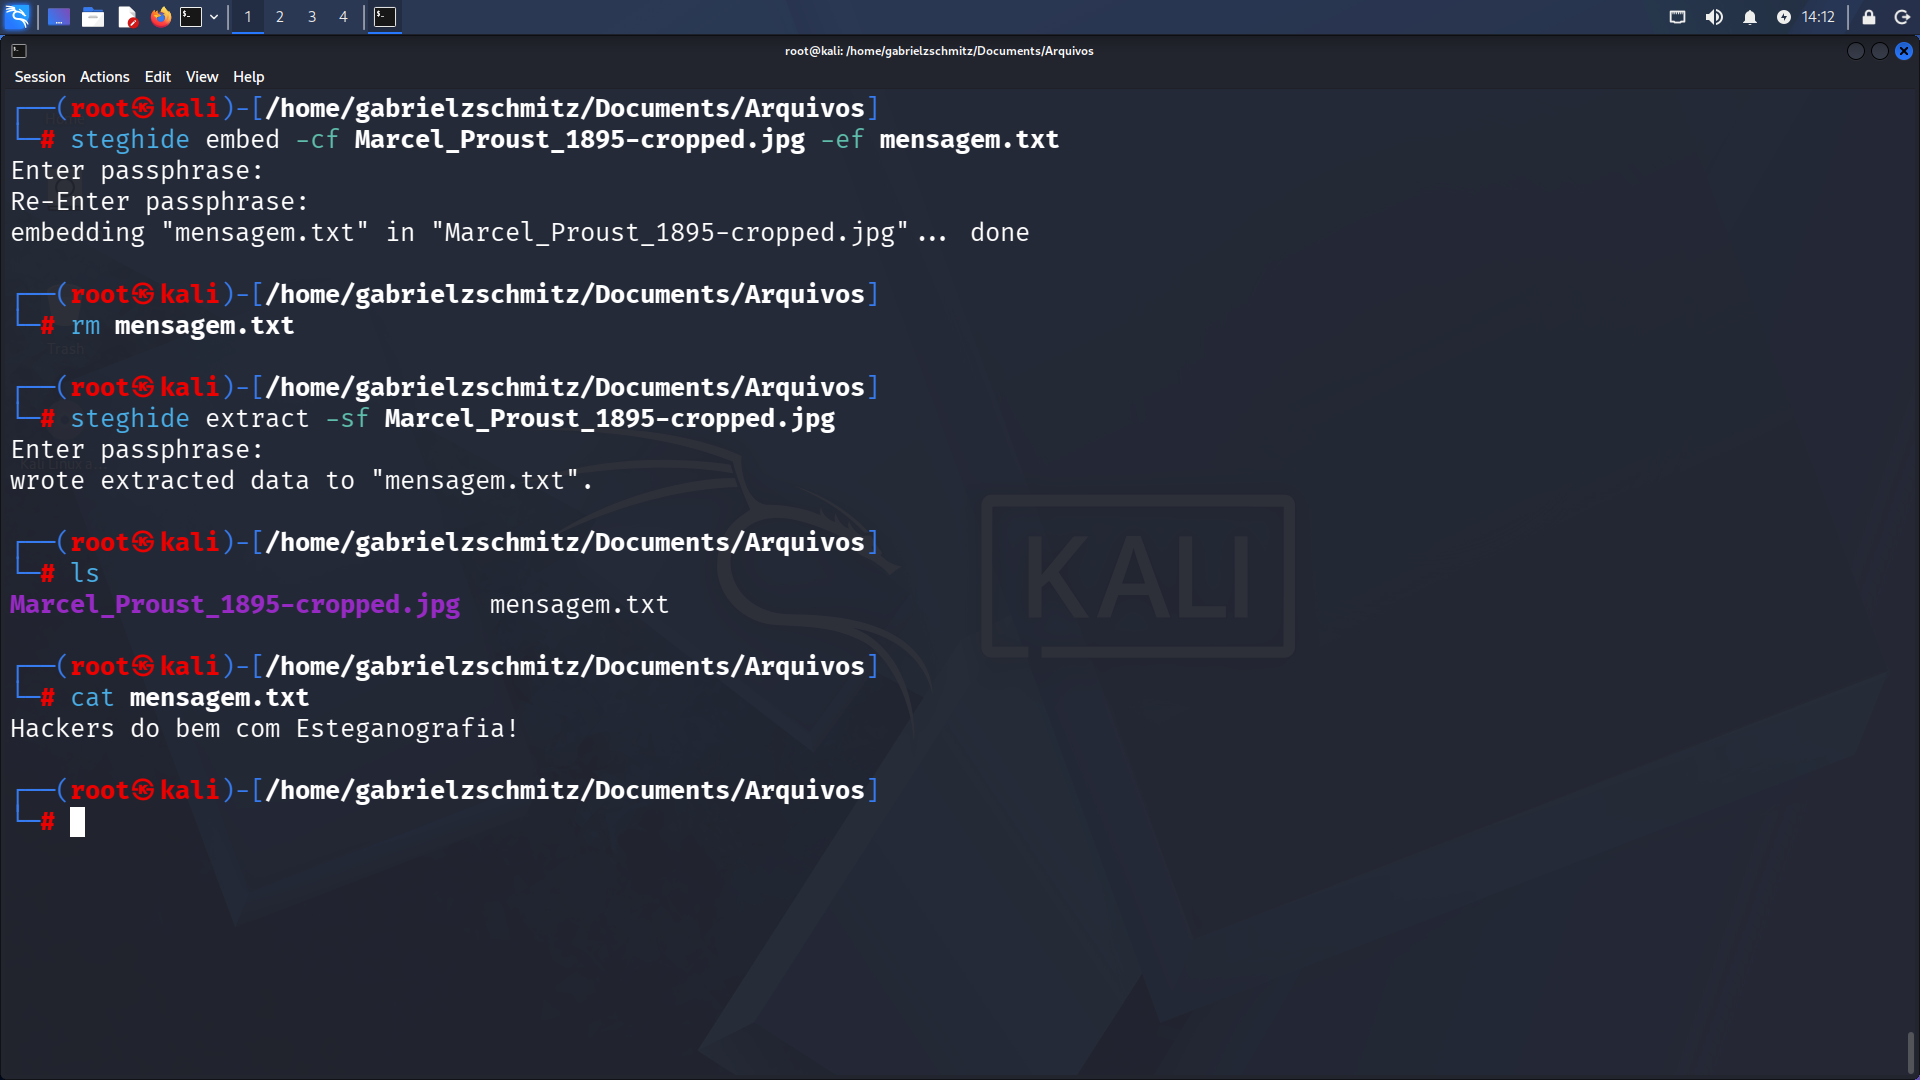
\includegraphics[width=0.99\textwidth]{./fig/fig8.1.png}
\caption{Recuperação do arquivo mensagem.txt oculto dentro da imagem utilizando esteganografia}
\label{fig:fig8.1}
\end{figure}

\newpage

\question[Atividade 8.2]{Ofuscação de Código Python}

\begin{figure}[H]
\centering
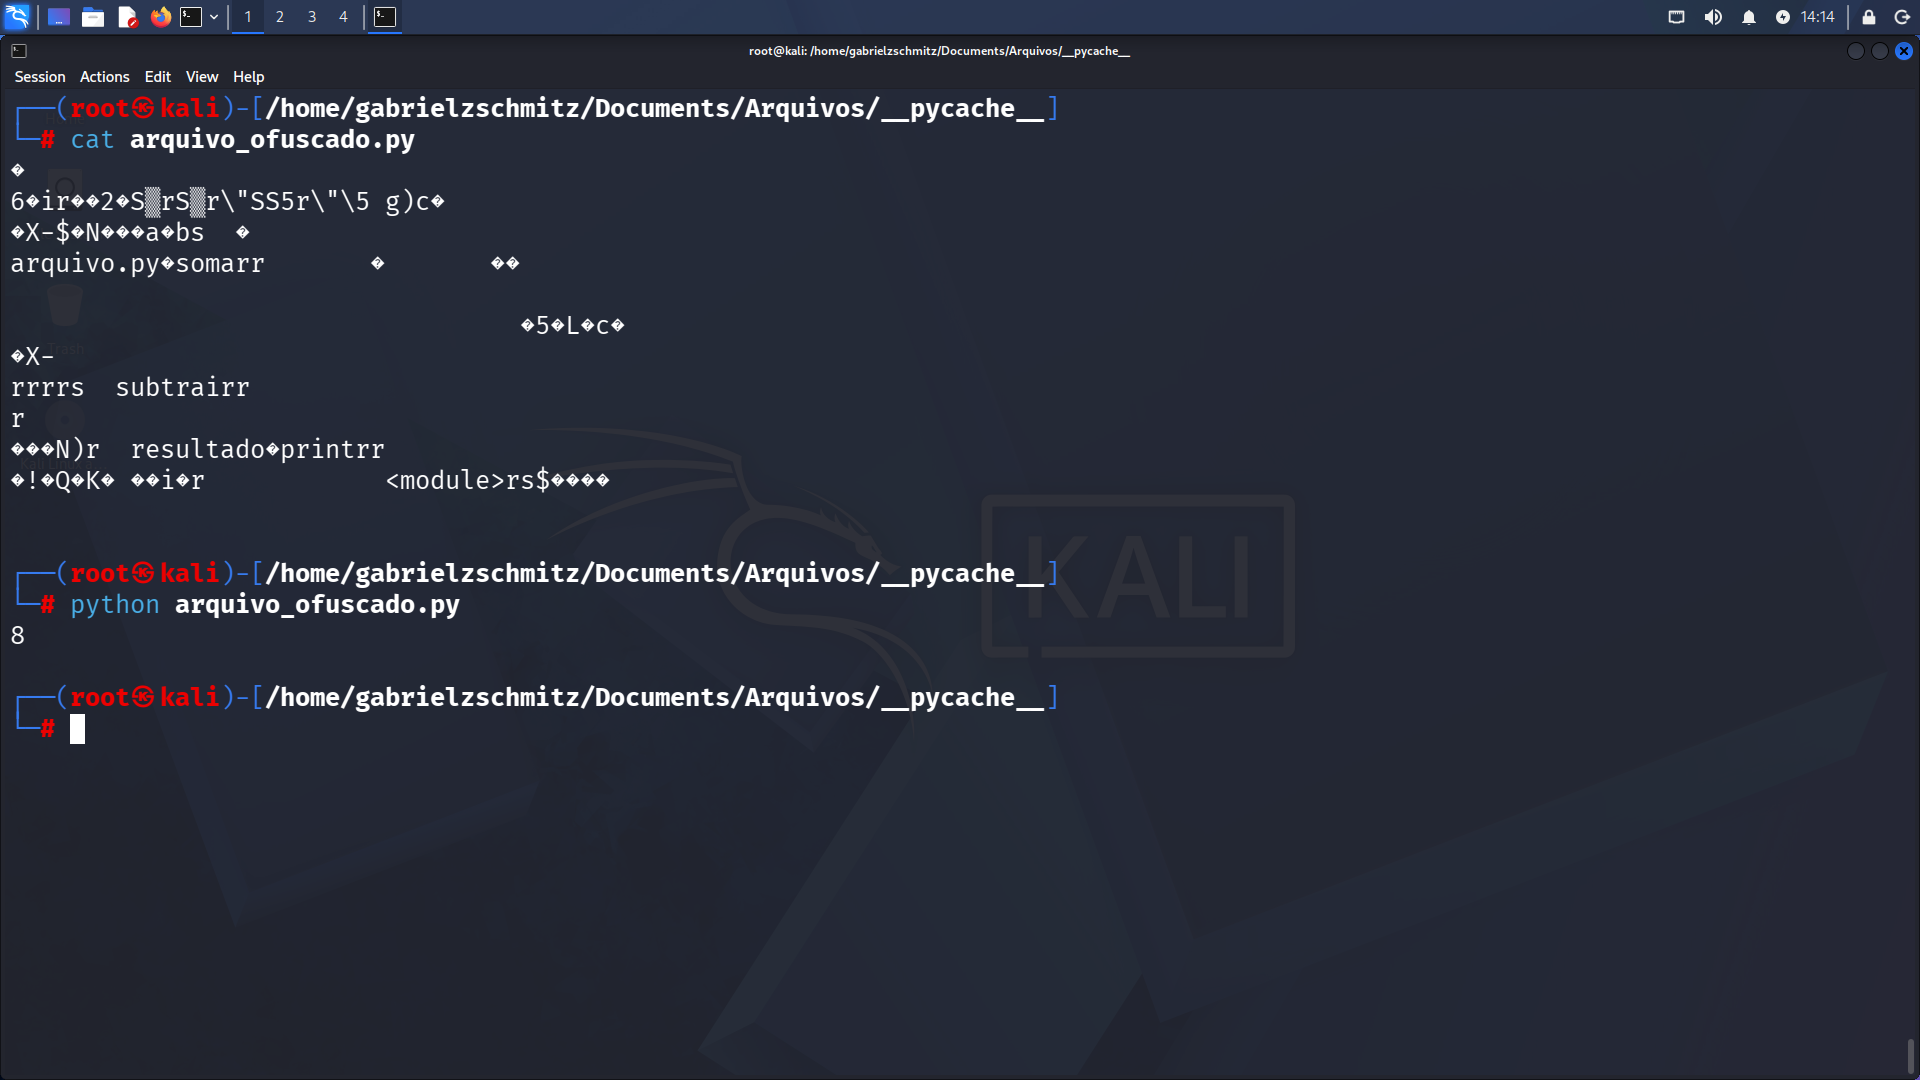
\includegraphics[width=0.99\textwidth]{./fig/fig8.2.png}
\caption{Execução do arquivo Python ofuscado gerado a partir do bytecode}
\label{fig:fig8.2}
\end{figure}

\newpage

\question[Atividade 8.3]{Criptografia com AES-256}

\begin{figure}[H]
\centering
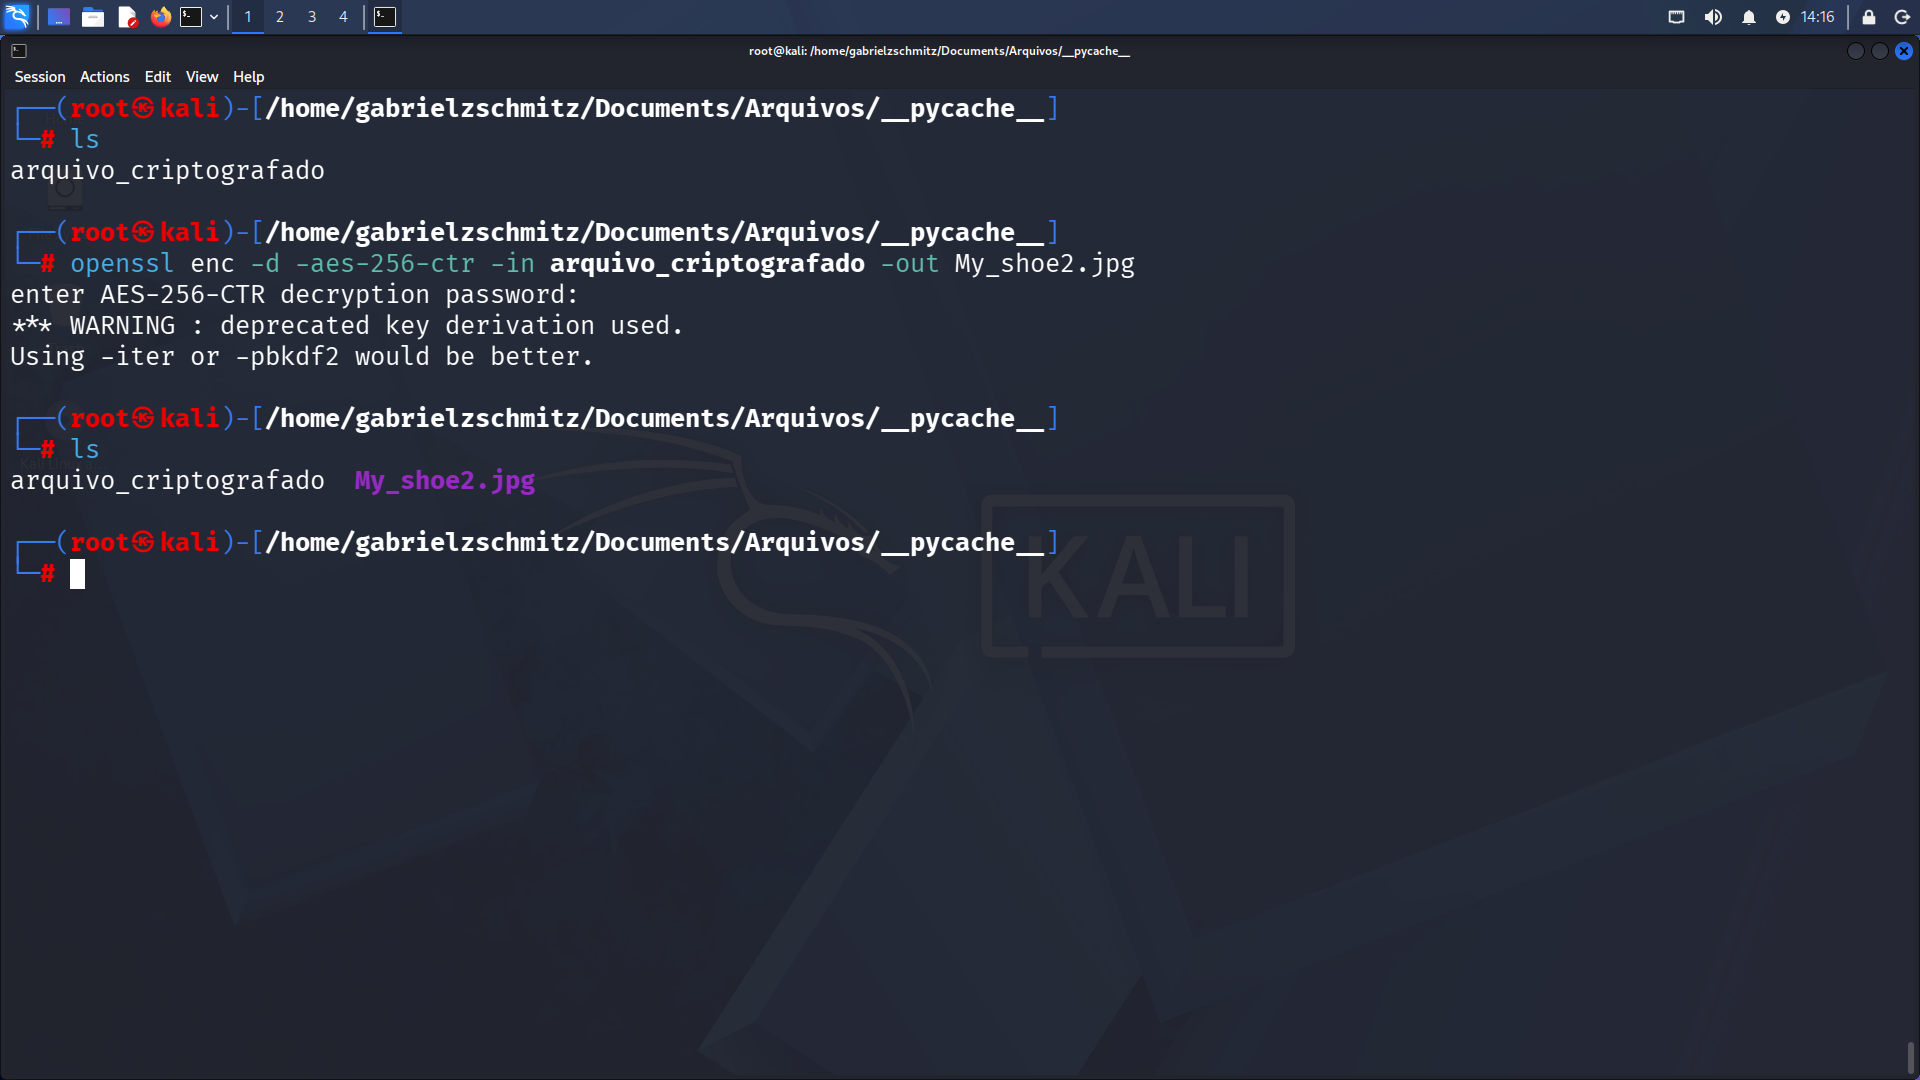
\includegraphics[width=0.99\textwidth]{./fig/fig8.3.png}
\caption{Decifragem do arquivo criptografado com AES-256 utilizando OpenSSL}
\label{fig:fig8.3}
\end{figure}

\newpage

\question[Atividade 8.4]{Criptografia com 3DES}

\begin{figure}[H]
\centering
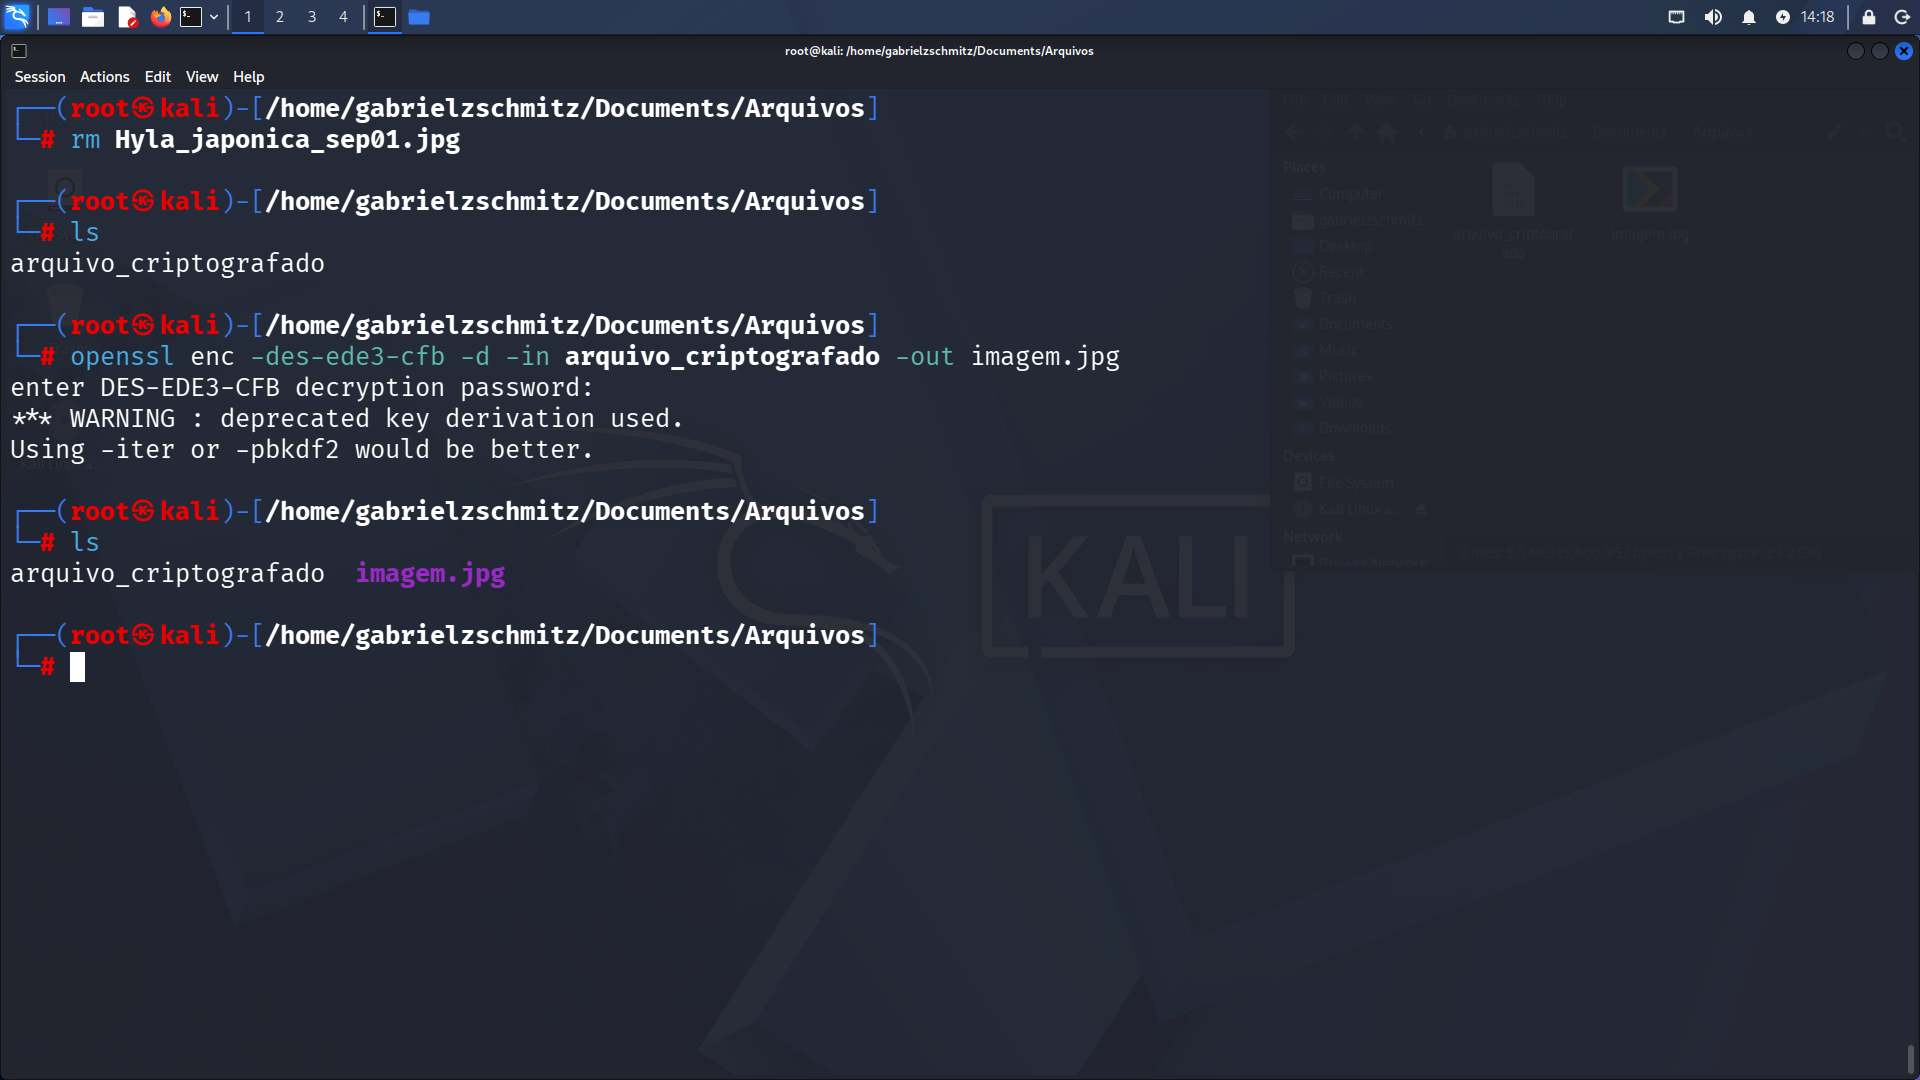
\includegraphics[width=0.99\textwidth]{./fig/fig8.4.png}
\caption{Decifragem do arquivo utilizando o algoritmo 3DES no modo CFB}
\label{fig:fig8.4}
\end{figure}

\newpage

\question[Atividade 8.5]{Criptografia com Blowfish}

\begin{figure}[H]
\centering
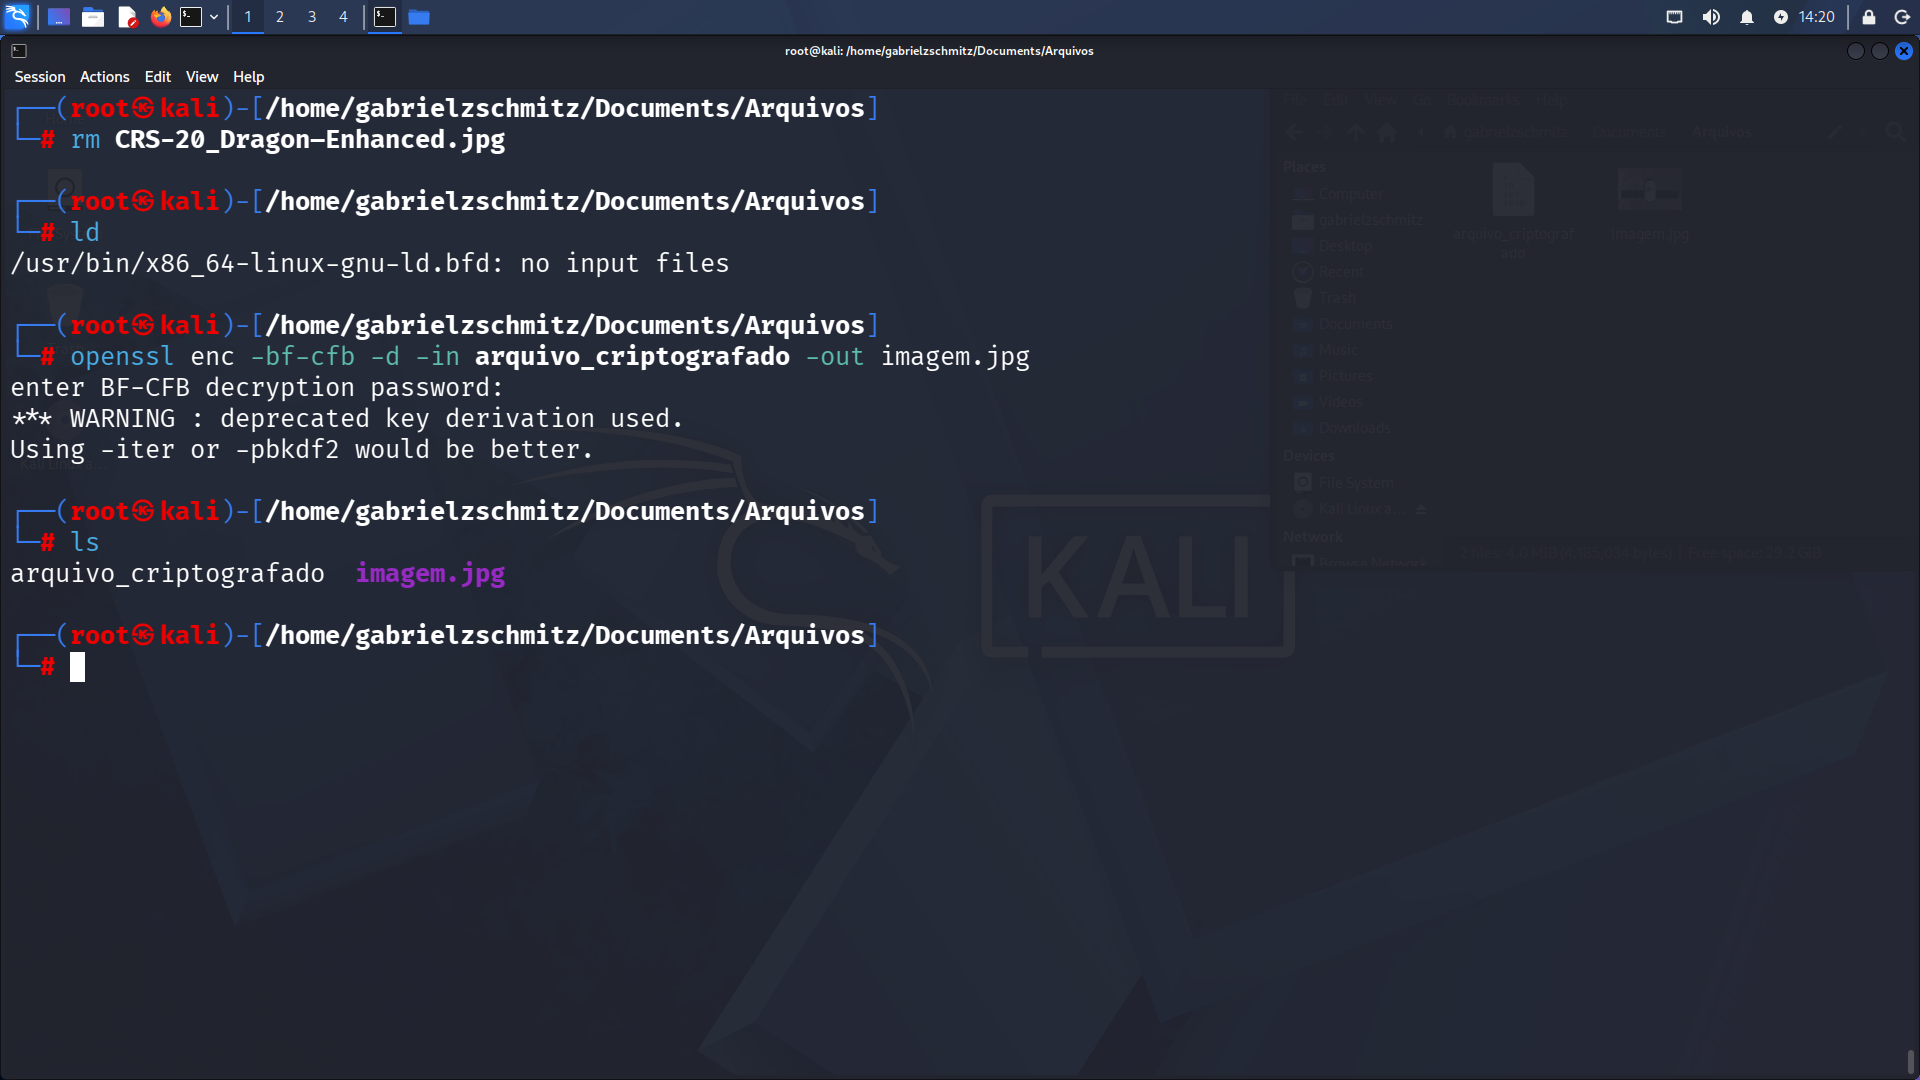
\includegraphics[width=0.99\textwidth]{./fig/fig8.5.png}
\caption{Decifragem do arquivo utilizando o algoritmo Blowfish no modo CFB}
\label{fig:fig8.5}
\end{figure}
